\PosterSection{1. INTRODUÇÃO}
\PosterBody
O monitoramento da qualidade da água em áreas remotas da Amazônia enfrenta conectividade intermitente, custos logísticos e restrições de energia. Avaliamos uma \textit{spiking neural network} (SNN) multimodal para predizer pH, oxigênio dissolvido (OD) e turbidez com inferência local e offline no Lago do Serpa, Itacoatiara--AM.

\begin{center}
\begin{minipage}[t]{0.47\linewidth}
\centering
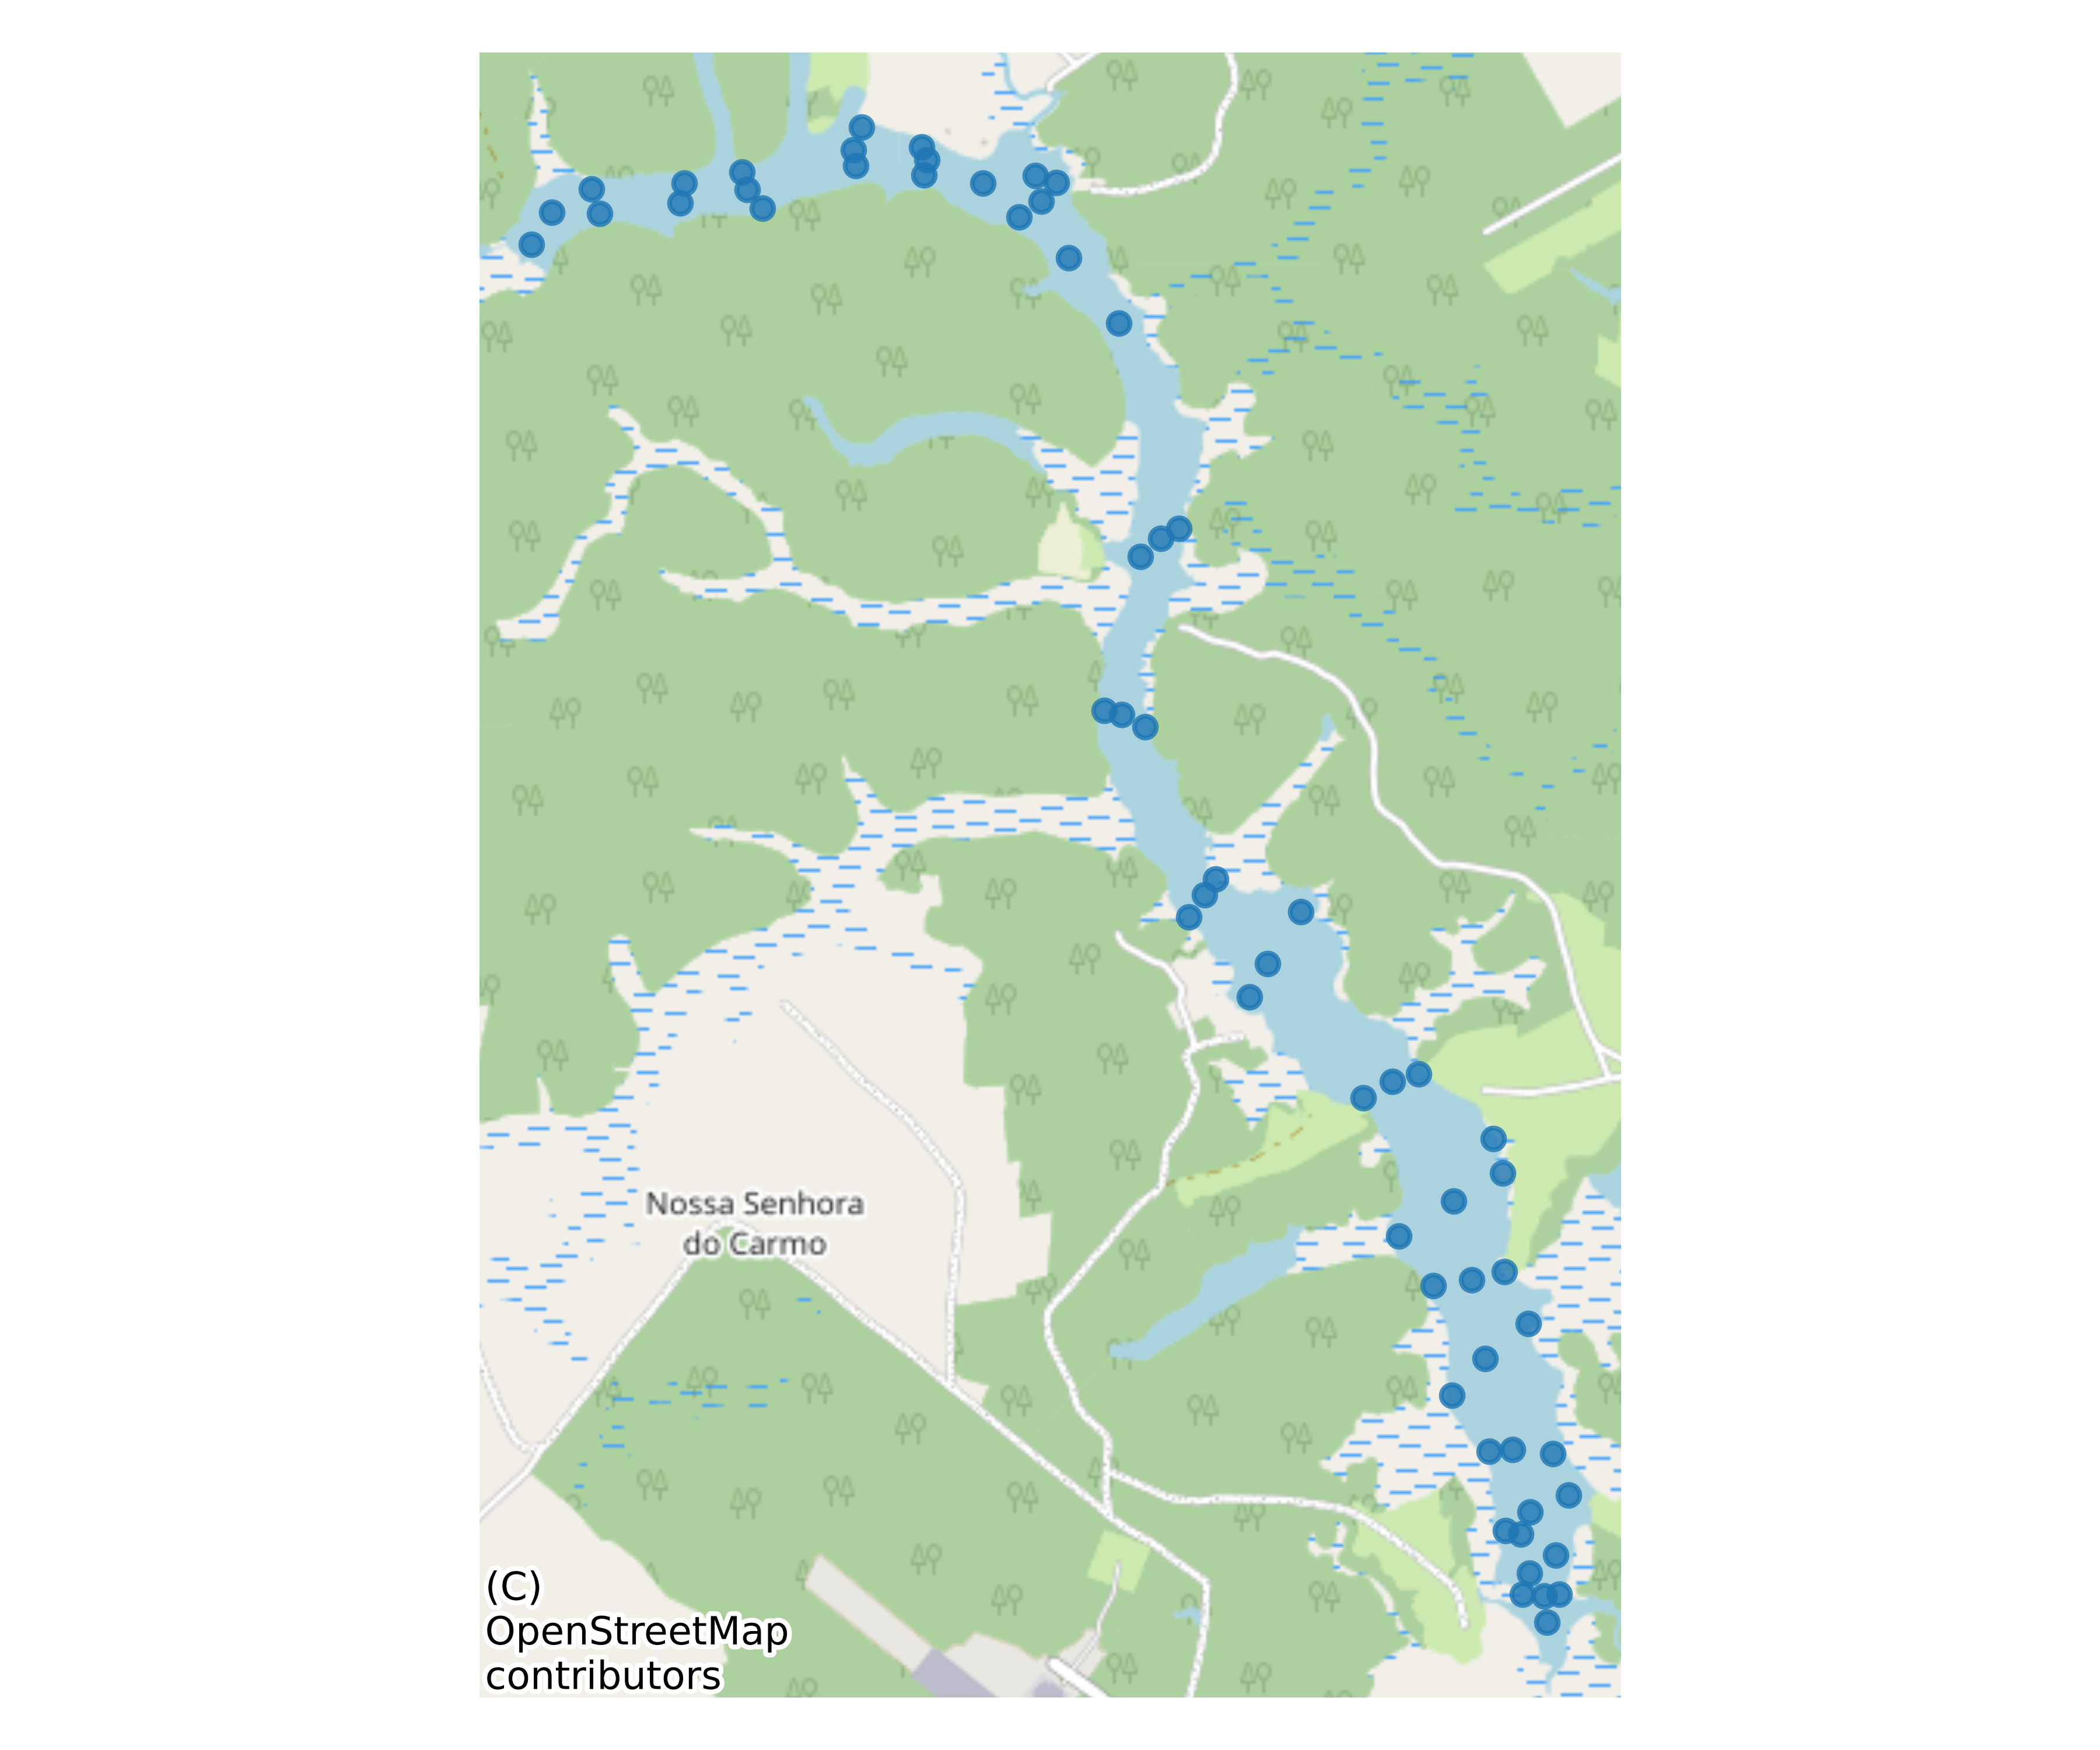
\includegraphics[width=\linewidth]{map_points_osm_21S.png}
{\PosterTiny\textbf{(a)} Pontos de amostragem\par}
\end{minipage}\hfill
\begin{minipage}[t]{0.47\linewidth}
\centering
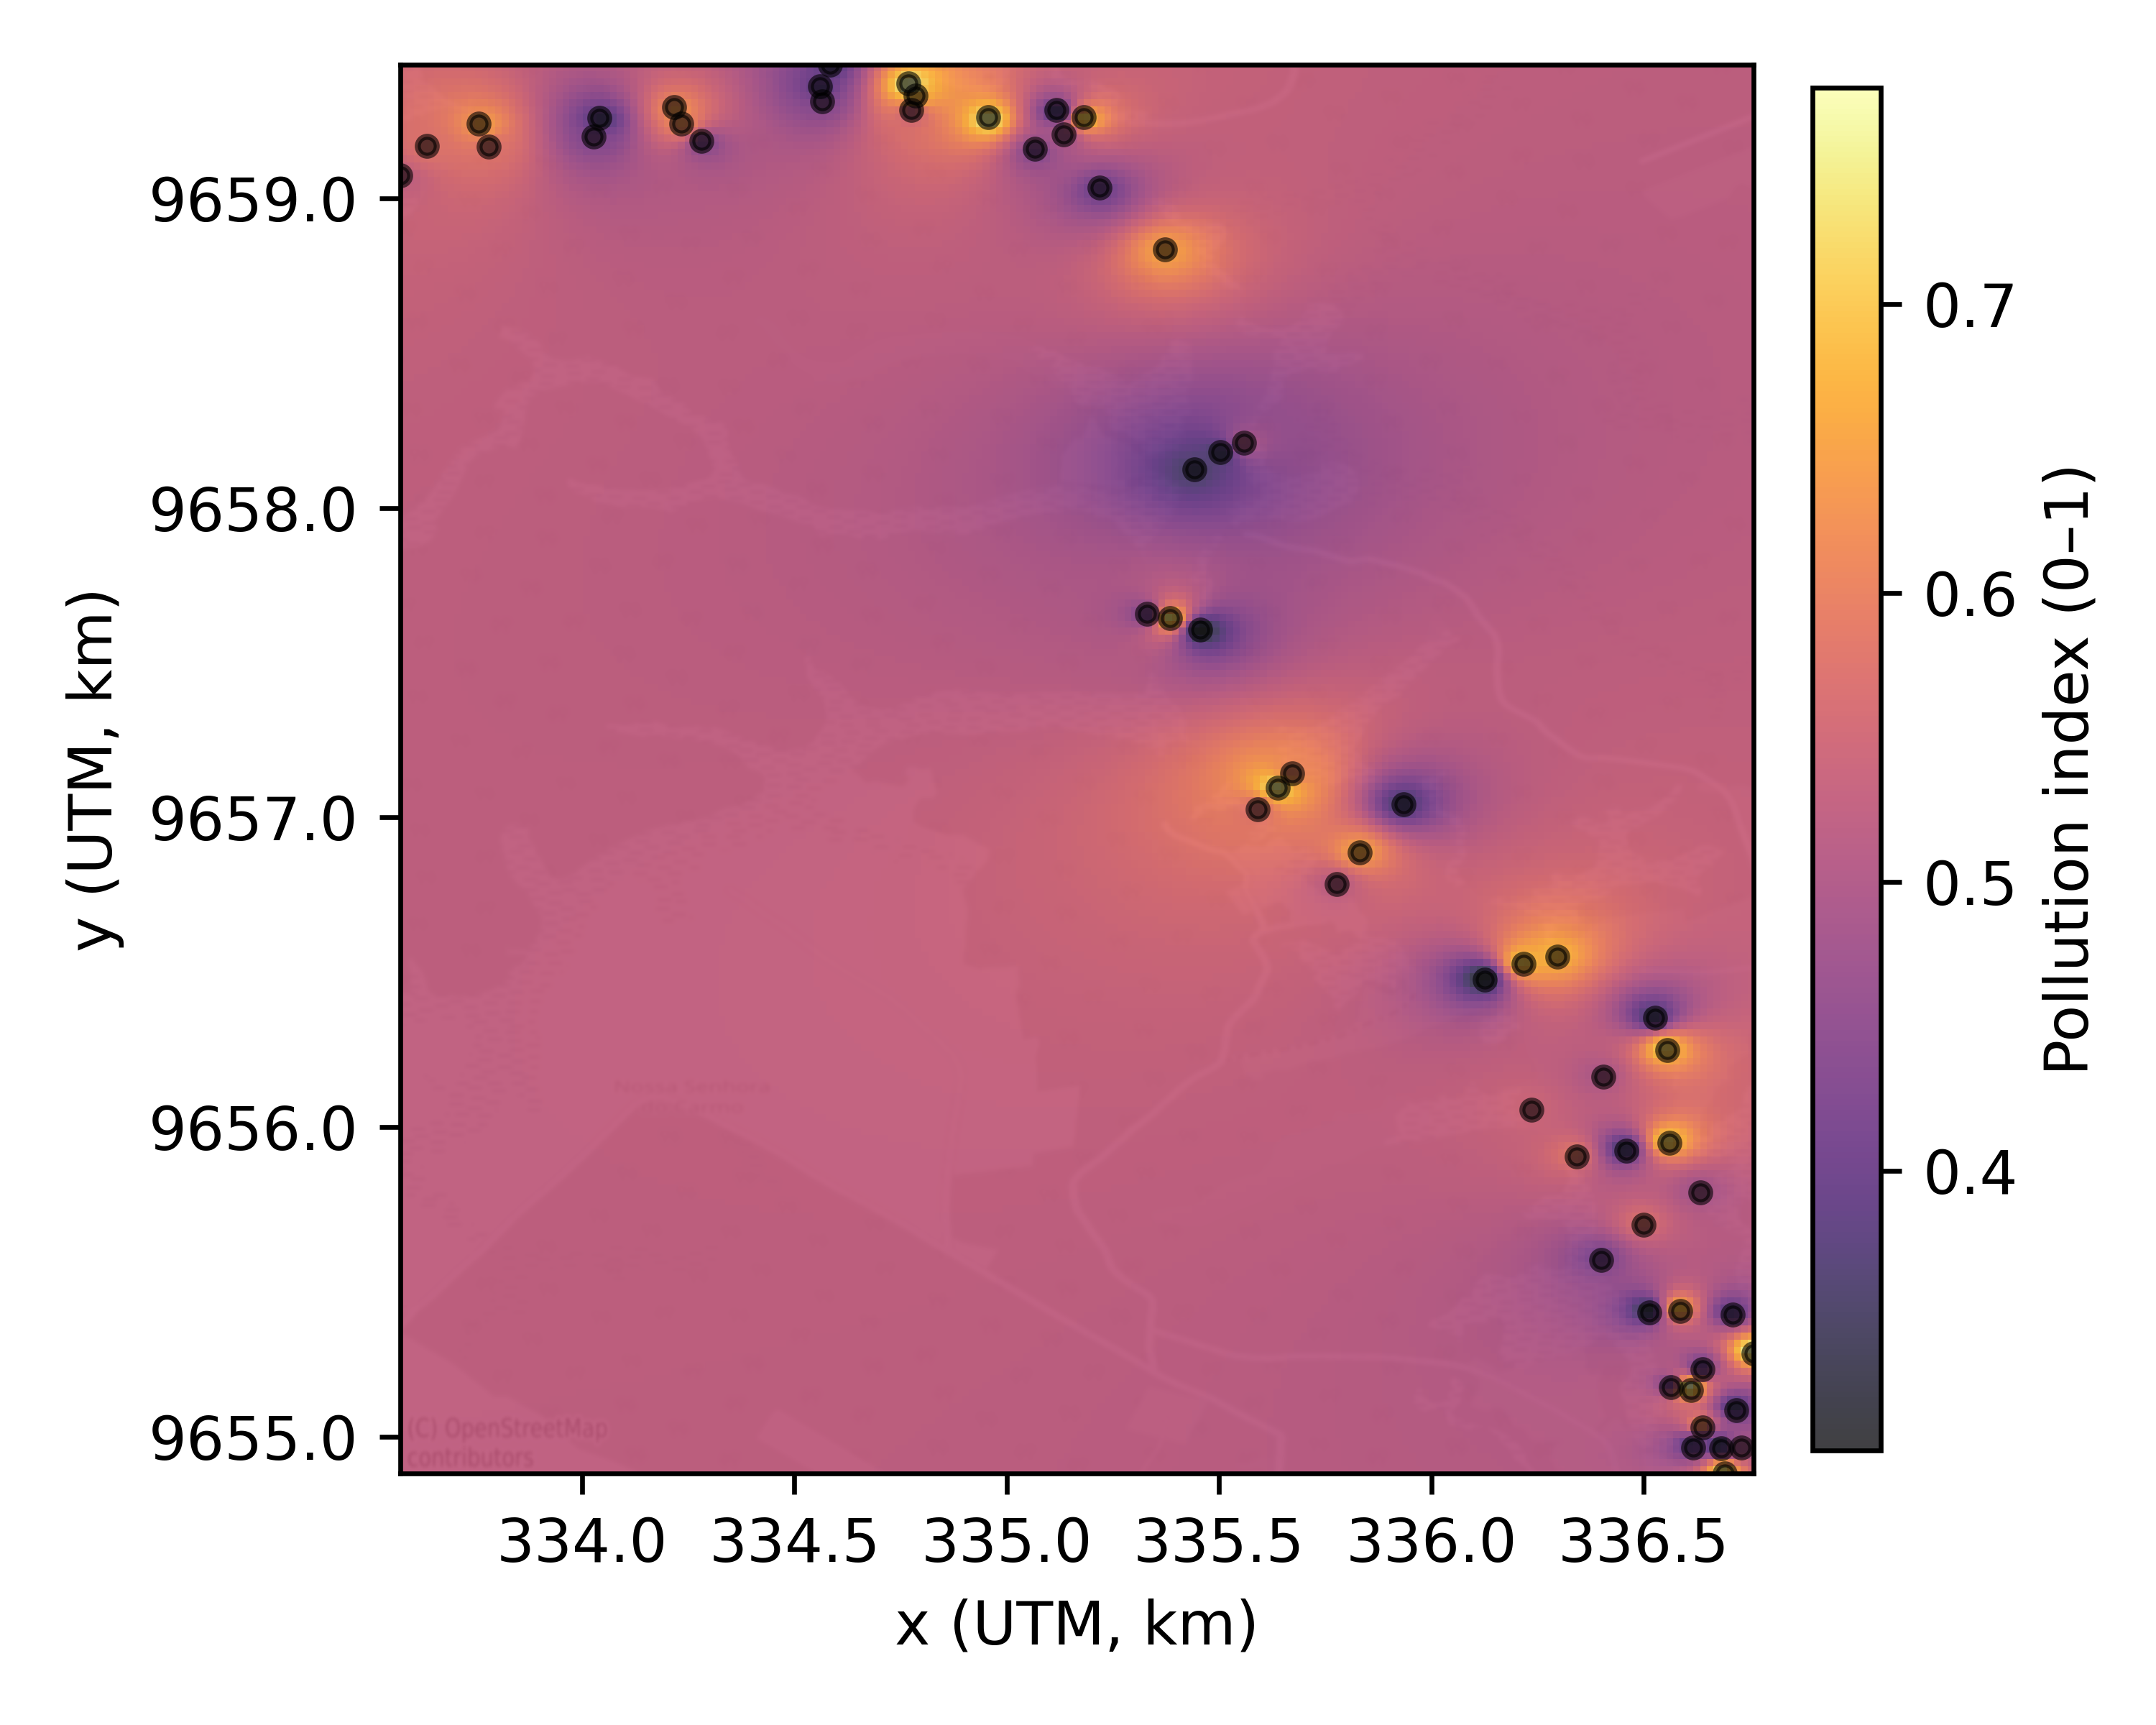
\includegraphics[width=\linewidth]{pollution_idw.png}
{\PosterTiny\textbf{(b)} Índice de poluição estimado\par}
\end{minipage}
\end{center}
{\PosterTiny\textbf{Figura 1.} Área de estudo no Lago do Serpa e representação espacial do índice de poluição composto estimado.\par}
\FigureSource{Dados de campo, interpolação IDW e base OpenStreetMap.}
